\chapter{Antecedentes}
\label{chap:antecedentes}
\section{Estudios experimentales sobre Intereacción Tangible}


\drop{E}l pensamiento computacional (CT) es un término calificado por Wing \cite{Wing} para describir un conjunto de habilidades de pensamiento, hábitos y enfoques que son integrales para resolver problemas complejos usando un sistema de computación y ampliamente aplicables en la sociedad de la información. Cada vez hay más consenso que el pensamiento computacional es una habilidad fundamental que todo el mundo necesita para tener éxito en nuestra cultura compleja y tecnológica. CT permite a los niños mejorar la capacidad analítica que puede ser útil tanto en ciencia, tecnología, ingeniería y matemáticas, y en muchas otras áreas profesionales, incluso en la vida cotidiana. 

Al exponer en edades tempranas a los niños a un pensamiento computacional ayuda a construir una base sólida en la mecánica de programación de computadoras. Grover \cite{Grover} toma la programación como una manera útil de que los niños aprendan la resolución de problemas y de pensamiento computacional. Las investigaciones indican que aprender a programar puede tener un efecto positivo y medible en el logro de los niños, no sólo en áreas como matemáticas y ciencias, sino también en habilidades del lenguaje, creatividad e interacción social y emocional. El hecho es que aun la programación para niños sigue siendo difícil y requiere de una fuerte motivación por parte del niño para tener éxito.

El entorno de programación debe motivar fuertemente al usuario, colocándolo en un contexto que sea tan convincente y significativo para el niño para que él/ella no se dé por vencido. Las interfaces tangibles ofrecen un entorno apropiado para este propósito ya que permite a los niños manipular “códigos” directamente, lo que hace que la programación sea más atractiva. Manipular objetos con las manos en lugar de modelos mentales puede cambiar la forma en la que un niño recuerda y recupera la información enseñada. Los niños entre 4 y 6 años aprenden a entender, representar y recordar objetos en su mente sin tener el objeto físico frente a ellos \cite{Piaget}.

Las interfaces digitales se convierten en poderosas herramientas de aprendizaje cuando los niños se convierten en creadores en lugar de sólo consumidores de contenido digital \cite{Resnick}. Al programar, los niños exploran los conceptos fundamentales de secuenciación, reconocimiento de patrones y relaciones de causa y efecto. Los niños aprenden a contar una historia de principio a fin, realizar secuencias de números y letras, formas o colores \cite{Kazakoff}.
Las interfaces de programación tangibles son especialmente adecuadas para la introducción de los niños pequeños a la programación desarrollando y aprovechando las estrategias de aprendizaje. El juego que implica la manipulación de objetos físicos que simbolizan otros objetos o ideas, permite a los niños explorar las reglas y sistemas de conceptos abstractos más amplios en diferentes ámbitos educativos \cite{Piaget}.

Los niños aprenden a contar una historia de principio a fin, secuencia de números y letras, formas o colores [5]. Las interfaces de programación tangibles son especialmente adecuadas para la introducción de los niños pequeños a la programación, ya que pueden coincidir con su habilidad de desarrollo. Aprovechan las estrategias de aprendizaje kinestésico natural de los niños para hacer que los conceptos abstractos sean accesibles e intuitivos \cite{Xu}. Mientras los niños juegan se involucran con el mundo físico haciendo uso de sus cinco sentidos \cite{Vygotsky}.
Los estudios realizados en adultos sobre el aprendizaje en entornos técnicos, han demostrado que las interfaces tangibles son más intuitivas de dominar al igual que más favorables a los comportamientos en resolución de problemas y apropiadas para fomentar la conciencia espacial, especialmente en usuarios con baja cognición espacial \cite{Quarles} \cite{Kim}.

¿El uso de interfaces tangibles estimula el aprendizaje en los niños pequeños?

Un ejemplo de ello, es un estudio sobre el aprendizaje de los alumnos de secundaria sobre las partes del cuerpo humano mediante una interfaz gráfica (representación en un ordenador) e interfaz tangible (partes de madera del cuerpo humano). Mientras la interfaz gráfica era más eficiente y promovía un aprendizaje más rápido de nuevos conceptos, al interfaz tangible promovía un compromiso más profundo y un enfoque prolongado explorando nuevas estructuras anatómicas \cite{Ploderer}.
En otro experimento que comparaba rompecabezas físicos y otros que fueron basados en pantallas, los niños de 7 a 9 años consiguieron realizar los puzles tangibles más rápidamente y con una colaboración de compañeros más directa que los que estaban computarizados \cite{Xie}.

Un estudio llevado a cabo por Horn \cite{Horn}, haciendo uso de un lenguaje de programación robótico tangible / gráfico, pudo demostrar que las interfaces tangibles eran más atractivas para los niños y más útiles para fomentar la colaboración. 

La interfaz tangible y la interfaz gráfica proporcionan un andamio estratificado a los niños mientras avanzan hacia un entorno de programación cada vez más auténtico. Horn describió el proceso de aprendizaje de programación de los niños como comenzando con un sistema tangible y luego transitando a un sistema gráfico con mayor capacidad y complejidad \cite{Bers}. La programación tangible se cree que es una práctica apropiada para el desarrollo de los niños pequeños \cite{McNerney}. En comparación con el funcionamiento de la computadora directamente mediante el uso del teclado y el ratón, el uso de objetos físicos para interactuar con la computadora es mucho más fácil para involucrar a los niños en el proceso \cite{McNerney}. Los niños pueden escribir programas montando los objetos físicos sin hacer uso pulsaciones en un teclado \cite{Horn}\cite{McNerney}.

Estos hallazgos han sido repetidos en estudios similares como el de Cheng \cite{Cheng} y el realizado por Manches y Price \cite{Manches}. Sin embargo, Horn \cite{Horn} reportó hallazgos de carácter únicos y exponían que la interfaz tangible parecía atraer por igual a las niñas y los niños (al contrario que la gráfica, que era más atractiva para los niños) y que se obtenían resultados sobre los niveles de comprensión y complejidad del programa que en este caso eran iguales tanto con la interfaz tangible como con la gráfica.

Son diversas las investigaciones realizadas sobre los beneficios que aportan a los niños el uso interfaces tangibles. Se realiza un análisis sobre diferentes estudios aplicados en este ámbito, mostrando el potencial de estos sistemas a la hora de promover el aprendizaje sobre los lenguajes de programación tangibles.

Amanda Strawhacker y Marina U. Bers \cite{Strawhacker} presentan los resultados de un estudio piloto realizado en tres aulas de jardín de infancia con tres tipos diferentes de interfaces para enseñar a los niños como programar un robot. Las interfaces utilizadas son: una interfaz gráfica de usuario (GUI), una interfaz de usuario tangible (TUI) y una interfaz en que los usuarios pueden cambiar libremente entre la entrada tangible y gráfica. Al proporcionar a los niños la opción de cambiar libremente entre interfaces, se le ofrece una herramienta de resolución de problemas. Manches y Price \cite{Manches} argumentan que cuando los niños se enfrentan desafíos en el proceso de diseño, es importante que puedan elegir que herramientas quieren utilizar para resolver el problema, lo que ofrece una ayuda para entender mejor el problema en sí mismo.

Los conceptos básicos a la hora de hacer el estudio, haciendo uso de una interfaz tangible se definieron de la siguiente manera:
\begin{itemize}
\item Secuenciación: este concepto introduce la idea de que el orden es importante al dar una serie de instrucciones, más específicamente, observar como el orden de los comandos afecta al orden de las acciones.
\item Repetición de bucles: Repetir loops permite explorar las acciones y secuencias que se repiten dentro de un programa, creando esencialmente programas dentro de otros más largos.
\item Programación creativa: Alentar a los niños a fijarse una meta imaginativa para su propio programa. Esto permite a los niños explorar todos los conceptos de programación aprendidos anteriormente.
\end{itemize}

Las cuestiones tratadas en esta investigación son: qué tan bien aprenden los niños con la tecnología (es decir, los lenguajes usados de programación en el contexto de la robótica) y qué tan bien aprenden los niños sobre la tecnología.
Los resultados obtenidos desvelan una mejora significativa entre interfaces TUI, GUI y HUI en tareas sobre bucles de repetición, siendo la interfaz GUI ligeramente más atractiva en tareas de secuenciación.
El estudio mostró que los niños usaban la interfaz tangible más que la gráfica cuando se les dio la oportunidad de usar ambas.

Un estudio realizado por Wang y Liu \cite{Wang_2015} resalta como ayuda la aplicación de sistemas tangibles a la hora de asimilar conceptos computacionales en actividades de programación. Para ello se tomaron participantes de edades comprendidas entre los 5 y 9 años. Se les facilito una serie de herramientas para la interacción, en este caso, una serie de módulos tangibles los cuales se han de colocar de una forma determinada para que los niños creen su programa con sus propias manos. El programa consiste en controlar un avatar virtual el cual se desplaza a través de un laberinto. Este laberinto es mostrado en una interfaz gráfica donde el niño puede ver los progresos conseguidos. Lo que se quiere obtener es como afecta estas interacciones en el pensamiento computacional de los niños, tomando especial interés a estos cuatro conceptos:
\begin{itemize}
\item Abstracción: La capacidad de abstracción consiste en encontrar el nivel adecuado de detalle para definir y resolver un problema \cite{Heureux}.
\item Automatización: Proceso por el cual se produce un ahorro de trabajo que se instruye para efectuar un conjunto de tareas repetitivas mediante una computadora. Es mucho más eficiente en comparación con el poder de procesamiento de un ser humano, por lo que las ejecuciones automatizadas de procesos realizados por máquinas simplifican el trabajo \cite{Guzdial}.
\item Descomposición y análisis de problemas: La descomposición puede tomar la forma de desmontar un problema a lo que se cree que es su esencia fundamental \cite{Lee}. Romper los problemas en partes más pequeñas para poder resolverlos y analizarlos de una manera más fácil, ayuda a la simplificación y resolución de problemas más complejos y de mayor escala.
\item Creatividad: La creatividad es a la vez una capacidad integral de los seres humanos y una parte importante del conjunto de actividades del pensamiento computacional \cite{Curzon}. Se intenta desarrollar la habilidad creativa de los niños estimulando su curiosidad, especialmente la imaginación.
\end{itemize}

¿Cómo toman forma estos cuatro conceptos CT para los niños en la programación?
Se propuso a los participantes realizar unas sesiones en las cuales debían completar unos niveles tanto de creación como de resolución de laberintos.
Los resultados obtenidos del estudio en las diferentes sesiones, mostraban como los niños eran capaces de formar sus propios programas mediante los bloques tangibles que les habían facilitado para la tarea, involucrándose en la creación y resolución de los problemas planteados. 

Durante las diferentes etapas se puedo observar como los niños necesitaban el proceso de abstracción para la reducir el problema. La abstracción también tuvo lugar cuando los niños diseñaron y crearon diferentes tipos de laberinto. 

En cuanto al concepto de automatización, la mayoría de los niños fueron capaces de indicar a sus distintos avatares que realizaran el recorrido, tomando especial entusiasmo cuando realizaban las ordenes que ellos les indicaban. 

En cuanto a la descomposición y análisis del problema los niños realizaron análisis cuando decidieron si el avatar se comportaba o no como se esperaba. Si el avatar estaba atascado o "mal encaminado", indicaba que su implementación de su idea de control es defectuosa o que algunos bloques estaban fuera de lugar. Creatividad. Para crear un laberinto, la programación se convirtió en un medio para la expresión personal y creativa de los niños. En el diseño de sus laberintos los niños involucraron sus fantasías y construyeron recorridos que iban más allá de los pensamientos comunes.

Se concluye que los sistemas tangibles tienen el prometedor potencial de ayudar a los niños a cultivar un cierto conocimiento del pensamiento computacional como abstracción, automatización, descomposición de problemas y análisis.

Teodosios Sapounidis y Stavros Demetriadis \cite{Sapounidis} realizaron una evaluación sobre el rendimiento de los niños con datos gráficos y tangibles en tareas de programación de un robot. El sistema propuesto está formado por dos subsistemas. El primero una interfaz GUI y el segundo una interfaz TUI.

El subsistema tangible consiste en bloques en forma de cubo que representan las estructuras de programación, tanto las simples como las avanzadas. Los usuarios conectan los diferentes cubos para así crear la programación del robot.

El subsistema gráfico consiste en un entorno de programación donde los participantes indican las operaciones a realizar por medio de la visualización de distintas estructuras, como; flechas, relojes, números…, que indican la acción a realizar por el robot.
Para la realización, se forman grupos de participantes de edades comprendidas entre los 6 y los 12 años para tal estudio.
Las tareas a realizar para la prueba, consisten en lo siguiente:
1. Realizar un programa secuencial simple de hasta seis ordenes (avanzar/retroceder, encender/apagar led, provocar un sonido) que implica el uso de varios cubos.
2. Formar un programa secuencial más avanzado que el anterior donde además de las ordenes descritas en la primera prueba, se añaden otras como girar a un lado y a otro.
3. Construir un programa secuencial que implique repeticiones (lazos).
Se les pidió a los niños realizar dichas tareas primero con una interfaz y luego con otra. Finalmente, después del proceso de interacción, se dejó a los niños utilizar libremente la interfaz que ellos quisieran. 

El tiempo usado en cada una de las pruebas realizadas a los diferentes grupos de niños objeto del análisis, muestran que los tiempos promedio utilizados para las tareas con la interfaz tangible, están por debajo de los tiempos utilizados para la gráfica.

El uso de la interfaz gráfica, ofrecio un porcentaje superior de error a la hora de ejecutar cada una de las tareas asignadas. La disminución del número de errores durante la programación del robot con el subsistema tangible se debe a la participación activa y a la motivación.
Por otra parte, la tarea de ejecución libre dejo los siguientes resultados:
Los niños de mayor edad, que eran usuarios de ordenadores, y por lo tanto, más experimentados, exploraron más órdenes y parámetros alternativos, y crearon programas más complicados con el subsistema tangible. Se produjeron menos errores de programación y se logró una mejor depuración en el caso tangible.
Por el contrario, los niños más pequeños pasaron casi el mismo tiempo en ambos casos, pero parece que eran más explorativos con los tangibles.

Se muestra una transición equilibrada de una interfaz a otra, en relación con la experiencia del usuario y el tiempo de interacción.
El estudio resalta que el uso de la interfaz tangible hace más probable que se lleve a cabo un proceso completo de depuración y corrección del error, mientras que con la gráfica es más probable que se descuide.
En conclusión, los resultados muestran que los sistemas tangibles aplicados en la programación, fomentan el aprendizaje y el rendimiento en tareas computacionales.


\section{Interacción tangible en la enseñanza de programación}

La educación tecnológica para los niños se está volviendo cada vez mas importante. Existe un desafío continuo para que los educadores desarrollen programas que reconozcan y respondan al impacto de la “revolución de la información”. Toman especial importancia para los niños pequeños, al poder explorar y dar sentido al mundo que les rodea, tener experiencias agradables y positivas con las computadoras y la tecnología. Existe la preocupación por la preparación física y cognitiva de los niños pequeños para usar las computadoras, y su impacto en su desarrollo social y educativo, que ha llevado a cierto rechazo de muchos educadores al uso de computadoras como un recurso educativo apropiado para la primera infancia \cite{Bailey}.
La cuestión es que los niños pequeños aprenden mejor mientras manipulan y transforman activamente materiales reales \cite{Beaty}.
Los niños pequeños deben ser capaces de desempeñar un papel activo en sus encuentros con la tecnología. Por ello el desarrollo de una interfaz tangible aborda este problema, ofreciendo una seria de beneficios en la educación y la creatividad. 

La finalidad es fomentar este sistema en el uso en aplicaciones para el escenario educativo, combinando para este propósito, las mejoras de los medios digitales utilizando entornos visuales, animaciones y sonidos, que son un importante estímulo a la hora del aprendizaje aumentando su motivación en tareas educativas.

Lo que nos ofrece el mercado en estos momentos en el ámbito de juegos con programación tangible o visual, se basa principalmente, en realizar una secuencia en la cual el niño establece previamente unas características y una serie de acciones a realizar sobre el juego, ya sea mediante un ordenador personal o dispositivo móvil haciendo uso de una pantalla para el desarrollo del juego, o mediante piezas pasivas colocadas con una determinada posición que indican las acciones a realizar en una secuencia.

A lo largo de la historia se han ido desarrollando aplicaciones de índole educativo para enseñar el lenguaje de la programación a niños pequeños, haciendo uso de interfaces tangibles. A continuación, se describen algunos de los proyectos enfocados al aprendizaje y enseñanza de la programación mediante la interacción tangible.

\textbf{Seymour Papert Turtle} \cite{Papert}. Fue uno de los principales promotores de la programación para niños mediante sistemas tangiblesPapert y sus alumnos del MIT\footnote{Computer Science and Artificial Intelligence Laboratory.}, comenzaron a investigar métodos para introducir a los niños en el mundo de la informática, para ofrecer maneras de programación de forma física. Esta investigación inicial, condujo a la creación del lenguaje Logo. Logo es un lenguaje de programación LISP. Este lenguaje es potente pero simple, y sirve para explorar la resolución de problemas lingüísticos y matemáticos. Logo es relativamente libre de las reglas sintácticas que hacen que muchos lenguajes de programación sean difíciles de aprender para los niños.

Su diseño consiste en un robot conforma de tortuga, el cual dispone de un mecanismo de dibujo. Este mecanismo fue diseñado para que los niños aprendieran conceptos geométricos. 
El centro de este enfoque, sostiene que los niños aprenden conceptos geométricos con mas facilidad, si pueden modelar formas geométricas en el espacio físico con su propio cuerpo. Este enfoque se denomina geometría centrada en el cuerpo. Por ejemplo, en lugar de pedirle inmediatamente a un niño que describa como podría instruir a la tortuga que dibujase una forma cuadrada, se le pide que explore la creación de la forma moviendo su propio cuerpo en el espacio sobre el suelo. A través de la prueba y error, el niño rápidamente se da cuenta de que caminar unos pasos, girar a la derecha 90º, y repetirlo cuatro veces, consigue realizar un cuadrado. Después de este ejercicio, el niño esta mejor preparado para programar la tortuga para repetir los movimientos. Estos movimientos, que previamente el niño había anotado, eran transmitidas al robot mediante un computador (ver Figura~\ref{fig:Papert}.

\begin{figure}[!h]
\begin{center}
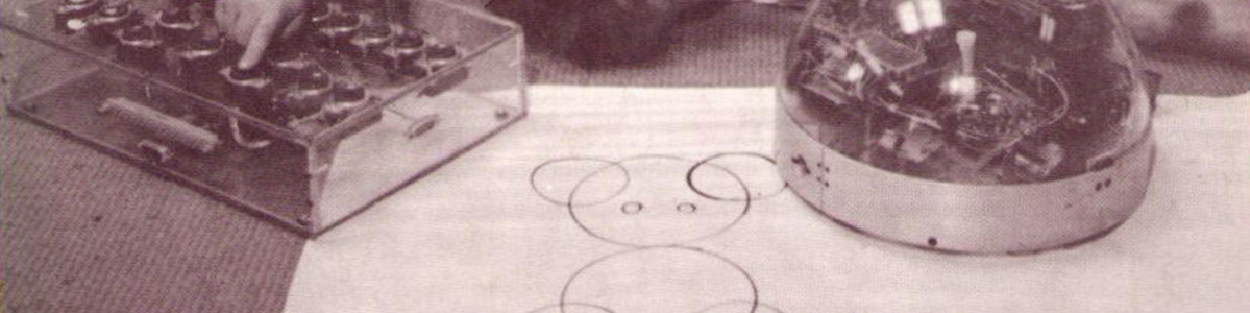
\includegraphics[width=0.5\textwidth]{Papert.pdf}
\caption{Seymour Papert Turtle. (Fuente: Mindstorms: children, computers, and powerful ideas \cite{Papert})}
\label{fig:Papert}
\end{center}
\end{figure}

\textbf{Tortis Slot Machine} \cite{Perlman}. 
Radia Perlman fue una de las pioneras en aplicar sistemas para el uso de lenguajes de programación en niños de 3 a 5 años, desarrollando la máquina Tortis. Durante años de enseñanza de Logo, se hizo evidente para los investigadores, que la mayoría de los niños no estaban preparados para comenzar a programar computadoras de la manera tradicional, es decir, tecleando el código de Logo en una computadora usando un teclado, hasta alcanzar al menos los 10-14 años de edad. 

Radia Perlamn a mediados de la década de los 70, creía que uno de los principales impedimentos para el acceso de los niños a la programación de computadoras no era solo la sintaxis del lenguaje, sino también la interfaz de usuario. Perlman comenzó a diseñar interfaces, que permitirían que incluso los preescolares, aprendieran a programar una tortuga. Para ello, se diseño dos nuevos dispositivos de entrada informalmente llamados \textit{Button Box} (Panel de funciones), y \textit{Slot Machine} (Máquina de ranuras). 

El panel de funciones sirve para indicar todas las operaciones a realizar, ya sea movimientos, encender o apagar una luz, etc. Los niños pequeños podrían usarlo como una especie de control remoto de televisión para decirle a la tortuga que hacer sin tener que aprender a escribir los comandos en un teclado. Este panel fue mejorado añadiendo un sistema de memoria, donde se puede registrar una transcripción de ordenes, para mas adelante realizarlas. Con ello, el niño podría mostrar físicamente al ordenador que hacer, para posteriormente realizar la secuencia.

Los dos grandes problemas encontrados fueron que los procedimientos eran demasiado abstractos para los niños pequeños. En segundo lugar, una vez iniciado el programa, no se permitía modificar la secuencia una vez grabada, por lo que el niño debía volver a realizar el programa. La solución fue la utilización de la Slot Machine. Esta máquina hace uso de tarjetas de plástico, que son insertadas dentro de ellas. La incorporación de estas tarjetas ofrecen la capacidad de manipular un programa directamente, mediante la adición, la reorganización y la eliminación de las tarjetas a mano.

A principios de los años 80, cuando las computadoras personales se hicieron mas comunes en las escuelas, los investigadores decidieron cambiar el enfoque de la tortuga moviéndose por el suelo, y adaptaron una representación de la tortuga por medio de la pantalla de un ordenador. La visualización de manera virtual en una pantalla, ofreció nuevas oportunidades de aprendizaje y exploración.

\begin{figure}[!h]
\begin{center}
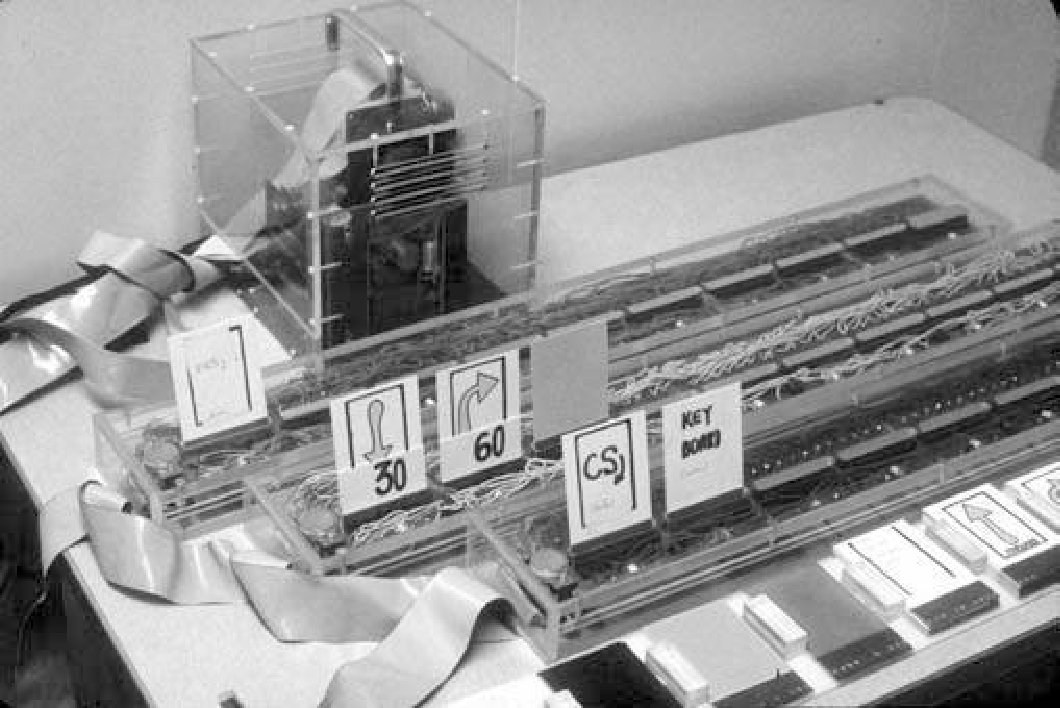
\includegraphics[width=0.5\textwidth]{Perlman.pdf}
\caption{Radia Perlman’s Slot Machine. (Fuente: Using computer technology to provide a creative learning environment for preschool children  \cite{Perlman})}
\label{fig:Perlman}
\end{center}
\end{figure}

\textbf{P-Brick} \cite{LegoLogo}. Hasta principios de 1990, no fue cuando los investigadores de la informática educativa del MIT, volvieron a estudiar la interacción con el mundo físico. La interfaz LEGO TC Logo, desarrollada por Steve Ocko, fue capaz de permitir a los desarrolladores, escribir programa Logo en un ordenador personal para controlar dispositivos construidos con bloques de construcción de LEGO. Estos artefactos podrían realizar tareas sorprendentes en el mundo real, como clasificar piezas LEGO por tamaños, aunque aun estos dispositivos estaban unidos mediante cables a la computadora. Martin, Sargent y Silverman, eliminaron este problema utilizando micro-controladores dentro de cada bloque, que ejecutaba el interprete de Logo.
P-Brick fue utilizado para controlar los primeros LEGO Mindstorms Robotics

\begin{figure}[!h]
\begin{center}
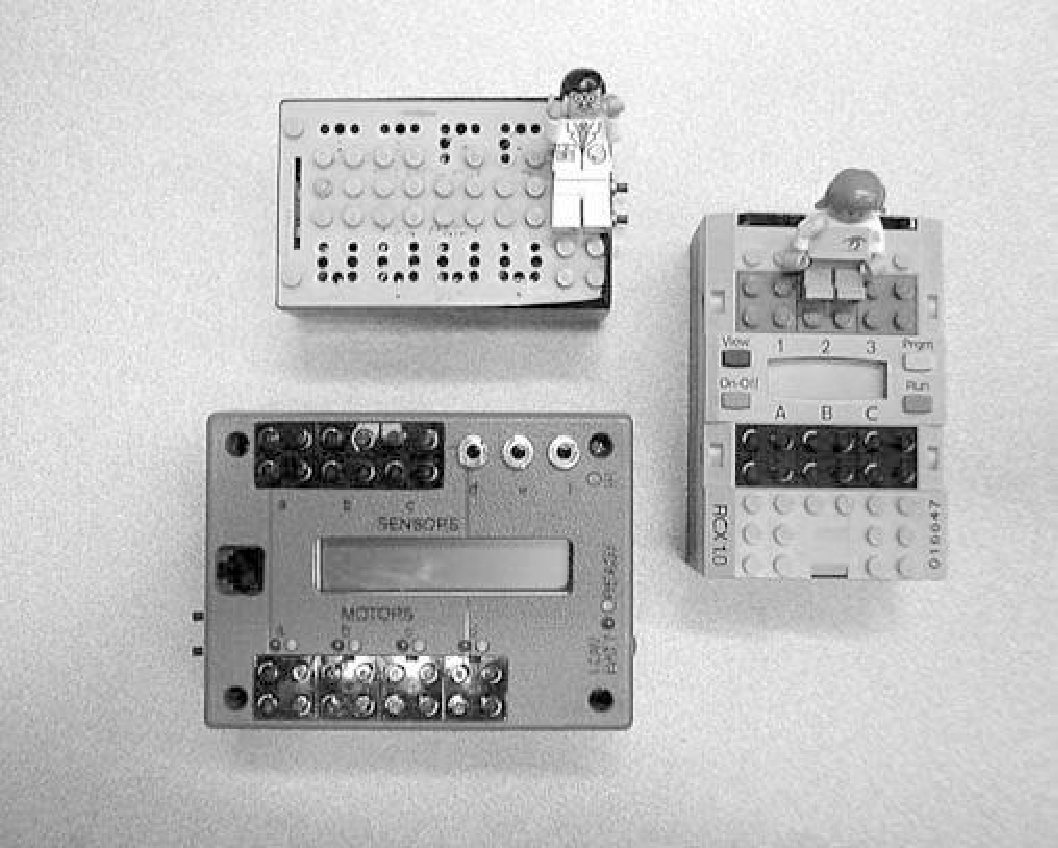
\includegraphics[width=0.5\textwidth]{PBrick.pdf}
\caption{Evolución de los bloques programables. (Fuente:\cite{McNerney})}
\label{fig:PBrick}
\end{center}
\end{figure}

P-Brick fue la inspiración y la base para una serie de juguetes diseñados para niños. \textbf{Dr.LegoHead} (Rick Borovoy), personaje interactivo, donde las partes de su cuerpo son removibles. \textbf{MyBot} lanzado en 2000, donde el juguete sigue la linea de componentes por bloques añadiendo nuevos sensores, como por ejemplo de inclinación, donde el juguete emite un sonido cuando es cambiado de orientación.
\textbf{Neurosmith Music Blocks}. Dispositivo donde el niño dispone de cinco bloques cúbicos coloreados, donde cada uno representa una nota musical, creando diferentes composiciones musicales.

\textbf{AlgoBlocks} \cite{Suzuki}. El Término “programación tangible” fue ideado por Suzuki y Kato, desarrolladores del sistema AlgoBlocks (Figura~\ref{fig:Algoblocks}). Este sistema estaba diseñado para la resolución colaborativa de problemas. Estaba formado por cubos relativamente grandes (15 cm), donde el objetivo del juego era guiar a un submarino a través de un laberinto. El lenguaje utilizado era bastante parecido a Logo. La programación era realizada físicamente por medio de los cubos que definían el recorrido a seguir para resolver el laberinto. La ejecución del programa era de manera virtual, representando las acciones gráficamente, mediante una pantalla de ordenador. Los bloques disponibles permitían realizar acciones como pueden ser giros o movimientos, incluso añadir parámetros. Otros bloques estaban diseñados para realizar sentencias de control como es: if-then-else y repeat-until, para un mejor control lógico. 


\begin{figure}[!h]
\begin{center}
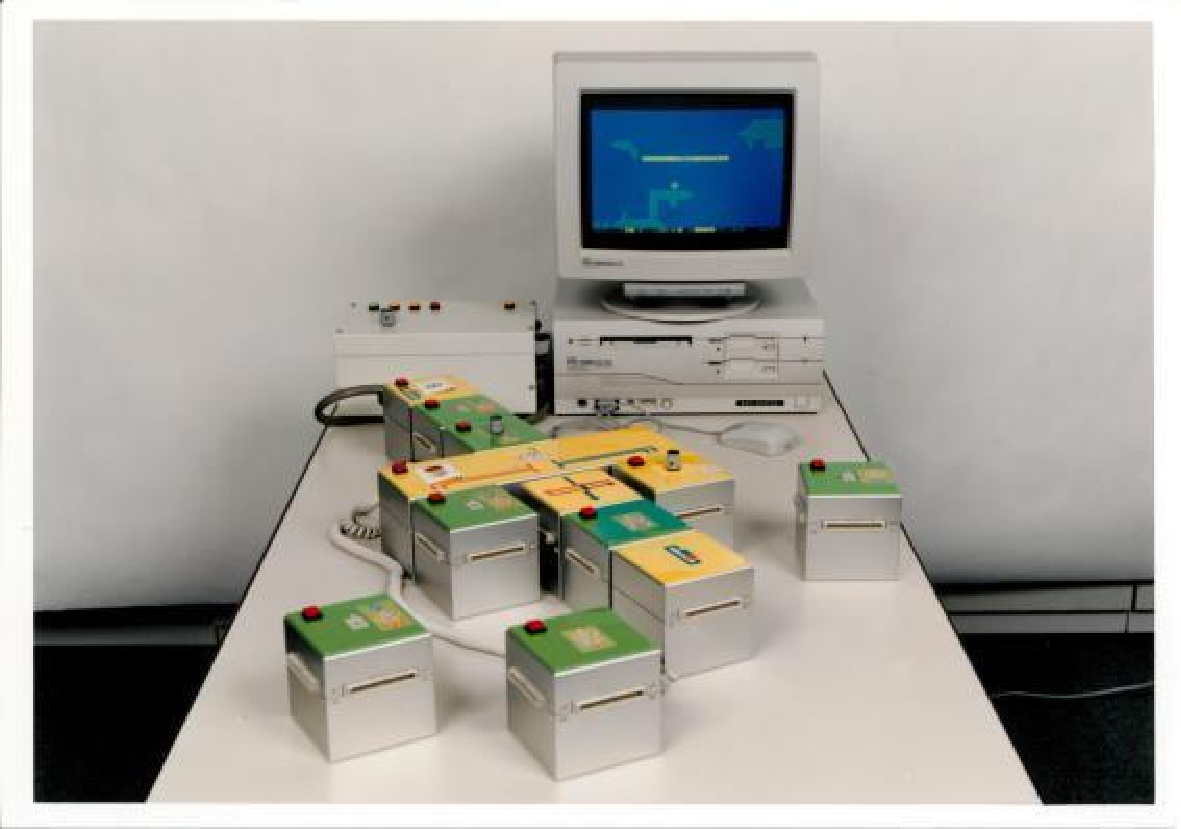
\includegraphics[width=0.5\textwidth]{Algoblocks.pdf}
\caption{Programación de un submarino en pantalla, usando el sistema AlgoBlocks. (Fuente: AlgoBlocks \cite{Suzuki})}
\label{fig:Algoblocks}
\end{center}
\end{figure}

\textbf{Digital Construction Set} \cite{McNerneyBricks}. En el año 2000, McNerney diseño esta plataforma para explorar lenguajes de programación tangibles que cumplieran ciertos requisitos de diseño: 
- Fácil de entender.
- Apropiado para realizar el juego de forma libre.
- Bloques simples que representen el vocabulario/léxico.
- Posibilidad de realizar un gran número de programas.
- Mejorar/depurar sin necesidad de herramientas externas.
El autor diseñó un sistema de ladrillos de LEGO apilables para construir los programas. El lateral de cada ladrillo disponía de una ranura donde el niño podía insertar elementos como ruedas digitales, botones analógicos, ademas de permitir definir parámetros, permitiendo así, una manipulación adicional (Figura~\ref{fig:Bricks}).
El sistema para comunicar y alimentar los, ladrillos se realizaba mediante contactos eléctricos (ISO 7816) en su parte superior e inferior, pudiéndose adaptar en orientaciones de 0 y 180 grados.
Cada bloque dispone de un microcontrolador PIC con un interprete Logo. Cada bloque era alimentado mediante una única batería que se situaba en el bloque de la base que formaba la pila de ladrillos. La comunicación entre ladrillos es mediante Bus serie I2C. 
Cada ladrillo se puede comunicar con sus vecinos, enviando mensajes que contengan eventos o datos. Un bloque vecino en la parte superior, puede recibir (y responder) mensajes de su vecino de abajo, produciéndose así, un flujo de datos ascendente.

\begin{figure}[!h]
\begin{center}
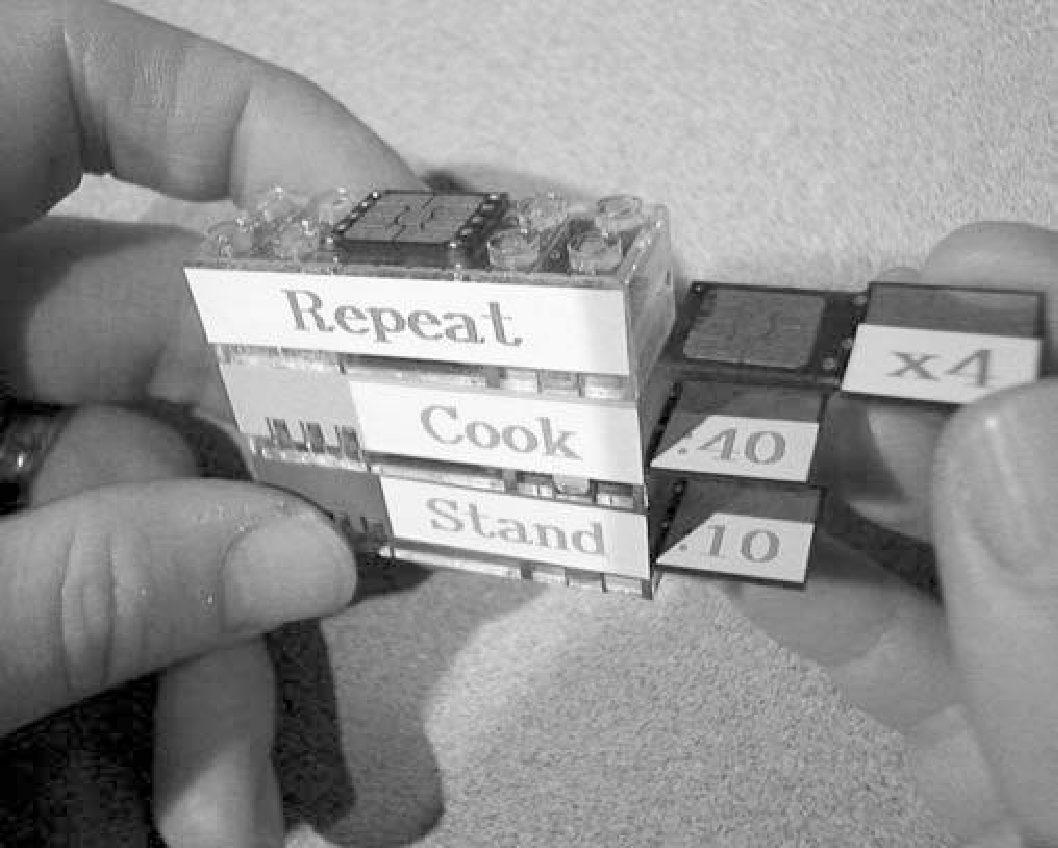
\includegraphics[width=0.5\textwidth]{Bricks.pdf}
\caption{Digital Construction Set. (Fuente:Tangible programming bricks \cite{McNerneyBricks})}
\label{fig:Bricks}
\end{center}
\end{figure}

Las característica más importante del sistema Digital Construction Set, es que permite a los investigadores y programadores jóvenes reprogramar el comportamiento de cualquiera de los bloques, permitiendo inventar su propio vocabulario especifico, adecuando cada uno de los bloques a una tarea particular.
No obstante, esta interfaz de programación tangible ofrece una limitación, ya que solo permite una construcción en una sola dirección, limitando así, posibles ramificaciones laterales en el programa.


\textbf{Electronic Block} \cite{Wyeth}. Este juego está formado por bloques, diseñados para que los niños puedan conectarlos unos con otros, siendo fácilmente apilables y enfocado principalmente para niños en edad preescolar, por lo que hace uso de una sintaxis fácil de programar. Dentro de cada bloque están situados diferentes componentes electrónicos para la interacción y realización del juego.
Existen tres tipos de bloques electrónicos:
\begin{itemize}
\item Bloques de sensores: Estos bloques son capaces de detectar luz, sonido y tacto. Son bloques de conector único, es decir, tienen una entrada del bloque anterior, y una salida al bloque de abajo. Para que los niños puedan identificar este tipo de bloque más fácilmente, todos ellos son de color amarillo.
\item Bloques de acción: Los bloques producen algún tipo de salida física, como puede ser encender una bombilla, emitir un sonido o reproducir una simple melodía. Existe un bloque de movimiento que emula un coche de cuatro ruedas que se mueve en línea recta.
El diseño de este tipo de bloques solo permite colocar otro bloque en la parte inferior. Estos bloques están adornados con iconos explicativos para su mejor utilización
\item Bloques lógicos:  Tienen un rol intermedio. Colocados entre un bloque sensor y un bloque de acción, tienen la capacidad de alterar la acción esperada. Los bloques lógicos proporcionan a los usuarios la capacidad de producir una acción si no se recibe un estímulo particular (not), producir retardos en las acciones (delay), solo producir una acción si las señales de entrada son recibidas simultáneamente (and), etc.
Cada bloque esta diferenciado por colores e iconos identificativos.
\end{itemize}

Estos bloques están diseñados para que los niños, jugando simplemente con ellos, puedan producir acciones y comportamientos, que les puedan parecer fascinantes. Pueden construir una torre que parpadea cuando hablan, o se mueve con un simple toque. La adicción de bloques lógicos añaden complejidad, y dan la posibilidad de crear una gran variedad de estructuras (Figura~\ref{fig:ElectronicBlocks}).

\begin{figure}[!h]
\begin{center}
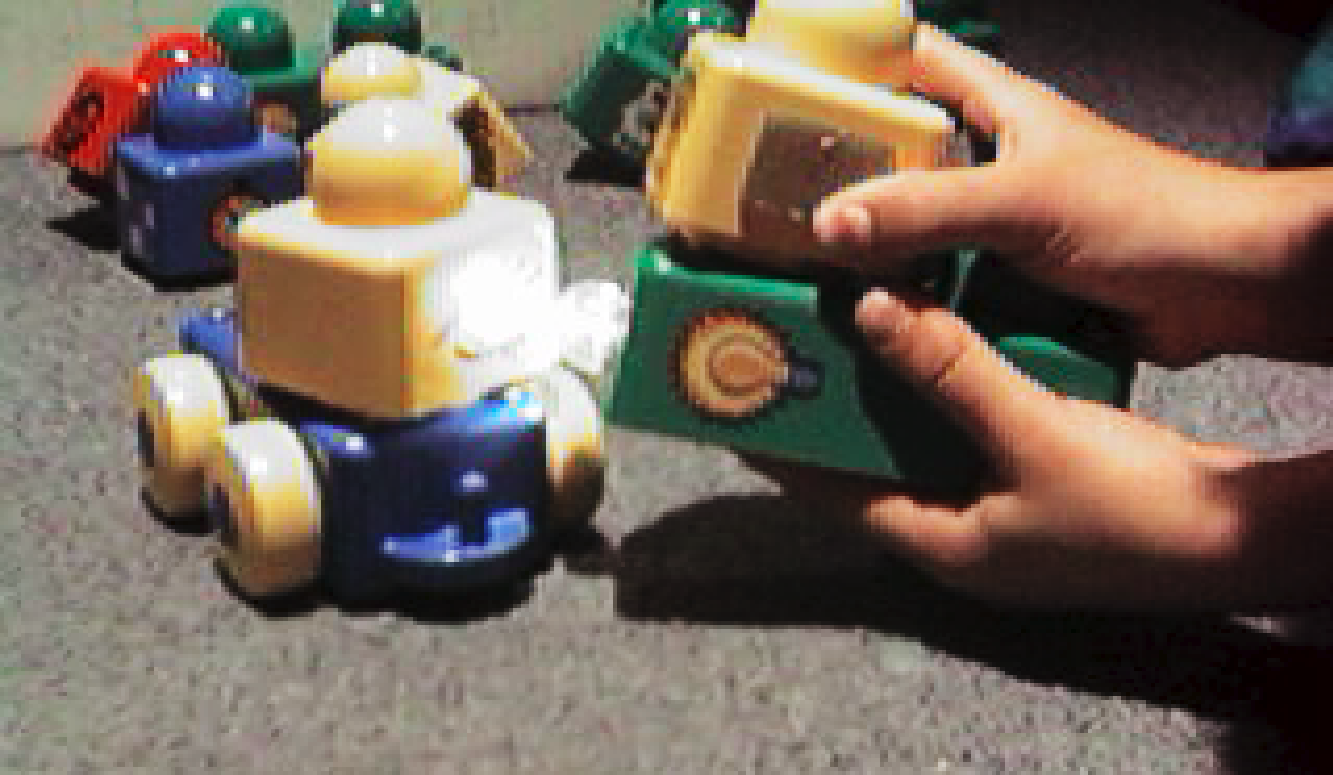
\includegraphics[width=0.5\textwidth]{Electronic_Blocks.pdf}
\caption{Lenguaje de programación tangible: Electronic Blocks. (Fuente: Tangible Programming Elements for Preschoolers \cite{Wyeth})}
\label{fig:ElectronicBlocks}
\end{center}
\end{figure}


D.Wang creador de \textbf{T-Maze} \cite{Wang_T-Maze}, posteriormente \textbf{TanPro-Kit} \cite{Wang_TanPro-kit}, y \textbf{E-BLOCKS} \cite{Wang_E-BLOCKS}. Estos sistemas de programación tangible utilizan bloques que, al conectarlos, generan en tiempo real movimientos dentro de un laberinto. En su funcionamiento se dispone de distintos tipos de bloques: bloque de inicio, bloque de fin, bloque de dirección y bloque sensor. Al interactuar los bloques, se muestra tanto en una pantalla, como en los propios bloques tangibles una realimentación (feedback), indicando si la acción llevada a cabo es correcta. Este tipo de TUI, no dependen de la representación "intangible" puesto que la retroalimentación activa a través de la representación tangible sirve como el canal de visualización principal.
En el caso de TanPro-Kit existe dos niveles de juego: un nivel introductorio, y un nivel adicional. Este sistema se centra en ayudar a los niños a aprender programación como principiantes. Ademas, no requiere de requisitos especiales a la hora de ser usado.


\begin{figure}[!h]
\begin{center}
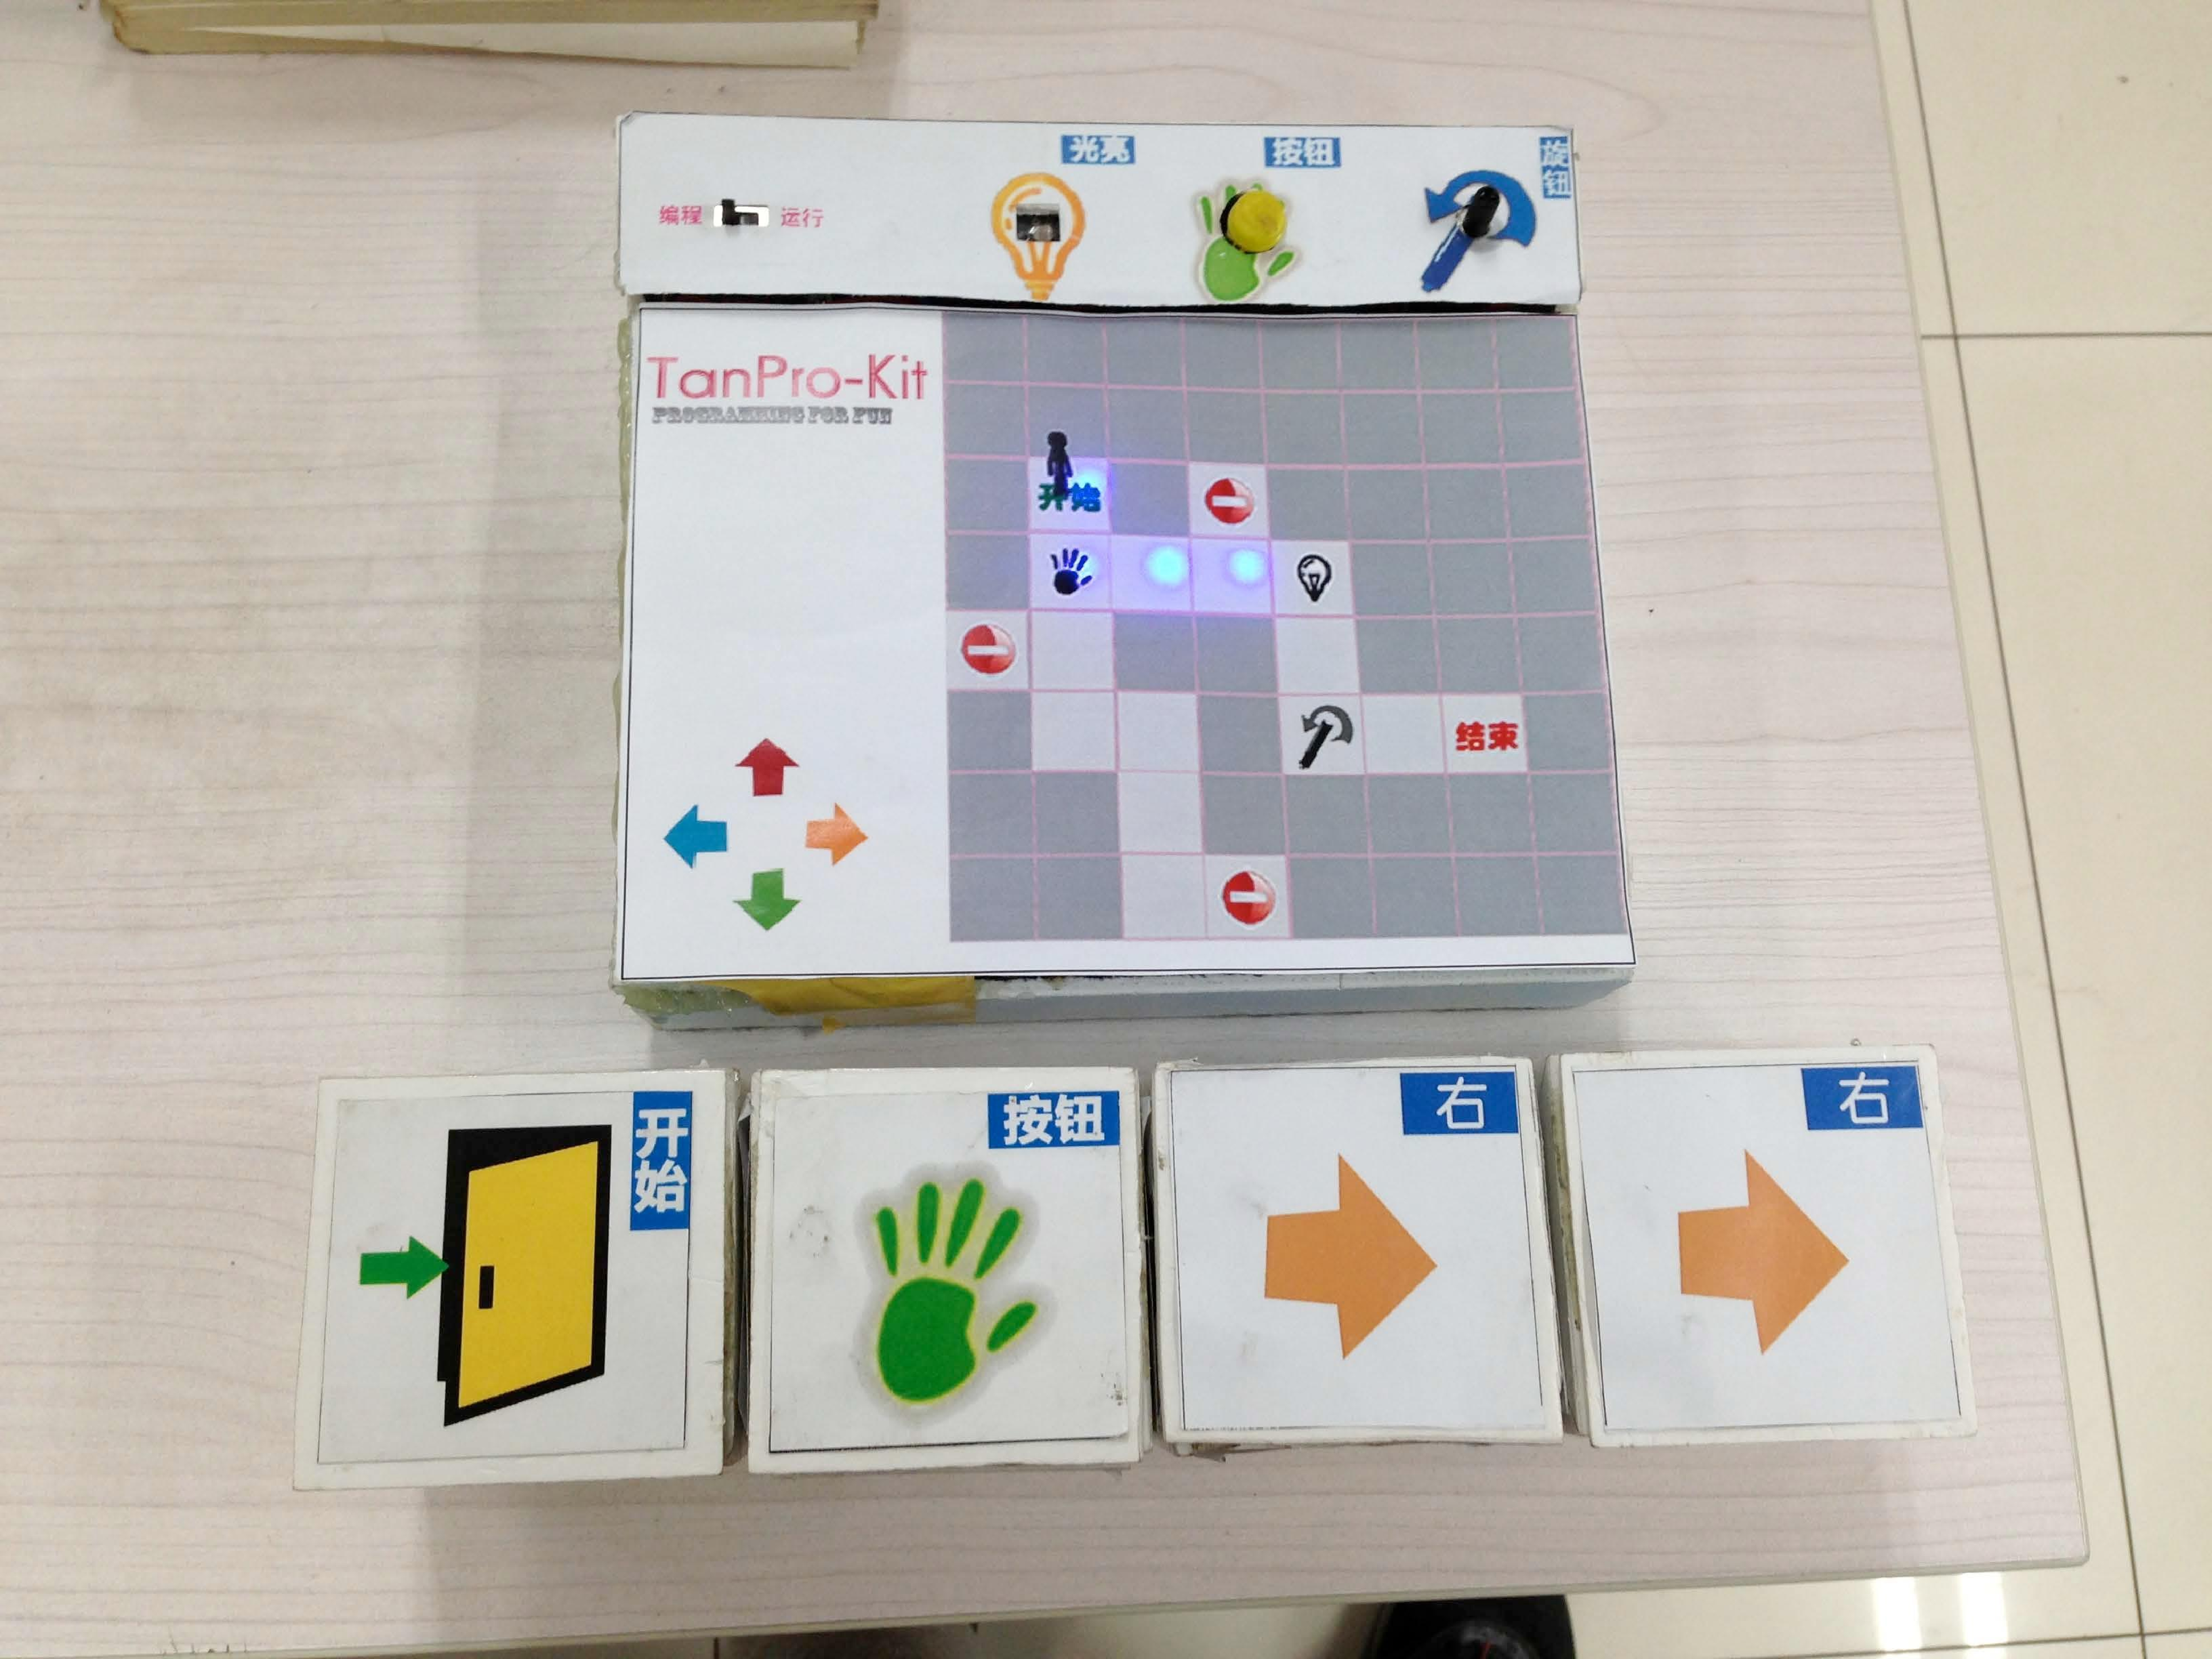
\includegraphics[width=0.5\textwidth]{TanProkit.pdf}
\caption{Caso básico de uso TanPro-Kit. (Fuente: TanPro-Kit: a Tangible Programming Tool for Children \cite{Wang_TanPro-kit})}
\label{fig:TanProKit}
\end{center}
\end{figure}


\textbf{Quetzal} \cite{Quetzal} es un lenguaje de programación diseñado para controlar LEGO Mindstorms\footnote{Línea de juguetes para niños enfocados a la robótica, que poseé elementos básicos para la progración de forma interactiva.}. Consiste en realizar el enclavamiento de varias piezas de plástico que representan las estructuras de control de flujo, acciones y parámetros. Las declaraciones en el lenguaje están conectadas entres sí para formar cadenas de flujo de control.
Al realizar un programa simple, se comienza con la instrucción Begin y termina con la instrucción End. En la Figura~\ref{fig:Quetzal} se puede ver un programa que inicia un motor, espera tres segundo para posteriormente detener el motor. Los usuarios pueden agregar o cambiar valores en los parámetros para ajustar tanto el tiempo de espera, como la potencia que genera el motor. Ciertas sentencias pueden aceptar valores de parámetros que pueden incluir constantes o lectura de sensores. Estos parámetros son representados mediante pequeñas fichas de plástico, que son insertadas en la cara superior de las piezas principales (declaraciones). El orden de las secuencias es un factor importante, pero la forma general de un programa no cambia su significado.

\begin{figure}[!h]
\begin{center}
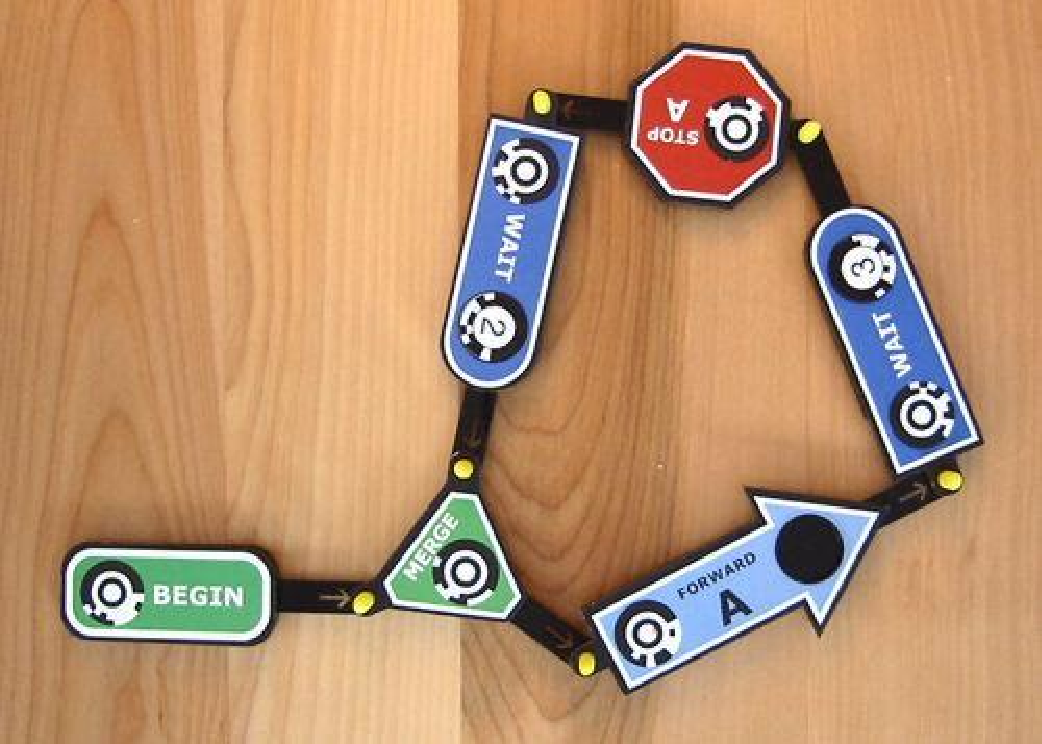
\includegraphics[width=0.5\textwidth]{Quetzal.pdf}
\caption{Ejemplo de programación de un bucle en Quetzal. (Fuente: Designing tangible programming languages for classroom use \cite{Quetzal})}
\label{fig:Quetzal}
\end{center}
\end{figure}

La implementación del programa es realizado por técnicas de procesamiento de imágenes, que convierten el programa físico en código de máquina. Cada sentencia es identificada según su posición, tamaño, o color. Las rutinas de procesamiento de imágenes utilizan un algoritmo de umbral adaptativo, que trabajan bajo diferentes condiciones de iluminación sin necesidad de calibración por parte del usuario. 

Una vez procesada la imagen e identificado cada una de las sentencias a realizar, el robot LEGO Mindstorms es accionado según las instrucciones especificadas.

\textbf{LEGO WeDo and Scratch} \cite{ScratchWeDo}. Scratch \cite{Scratch} es un lenguaje de programación visual basado en Logo, diseñado para que los niños creen fácilmente su propio contenido interactivo (juegos, música, historias interactivas,…). Ademas, Scratch facilita una pagina web donde los niños pueden subir sus propias creaciones y compartirlas, fomentando de esa manera, el trabajo en colaboración. Incluye funcionalidades, interfaz gráfica, multimedia, eliminación de errores de sintaxis, etc. Permite usar programación dirigida por eventos con objetos activos denominados sprites. Estos sprites pueden dibujarse como gráficos de tipo vectorial o mapa de bits, o pueden ser importados desde fuentes externas incluyendo webcams. Una vez creado un objeto, éste puede ser manipulado aplicando bloques de funciones que van desde el movimiento, apariencia, sonido,… y controlados mediante bloques de eventos, operadores, etc.

El conjunto de construcciones WeDo \cite{WeDo}, permite a los usuarios la construcción y programación de modelos simples de LEGO mediante el uso de una computadora.

La combinación de Scratch y WeDo en la creación de proyectos dedicados a la robótica, ejemplifica el paradigma del aprendizaje del construccionismo\footnote{Teoría de la educación basada en la teoría del aprendizaje desarrollada por el sicólogo suizo Jean Piaget \cite{Piaget}} \cite{Papert}, donde el joven estudiante es el protagonista del proceso de aprendizaje. El construccionismo afirma que la programación, depuración, el acto de construir un sistema, encontrar problemas y resolverlos, es la manera mas eficaz de que un niño aprenda. Las dos plataformas (software y hardware), facilitan la introducción de la programación y la robótica en la escuela primaria (Figura~\ref{fig:ScratchWeDo}).

\begin{figure}[!h]
\begin{center}
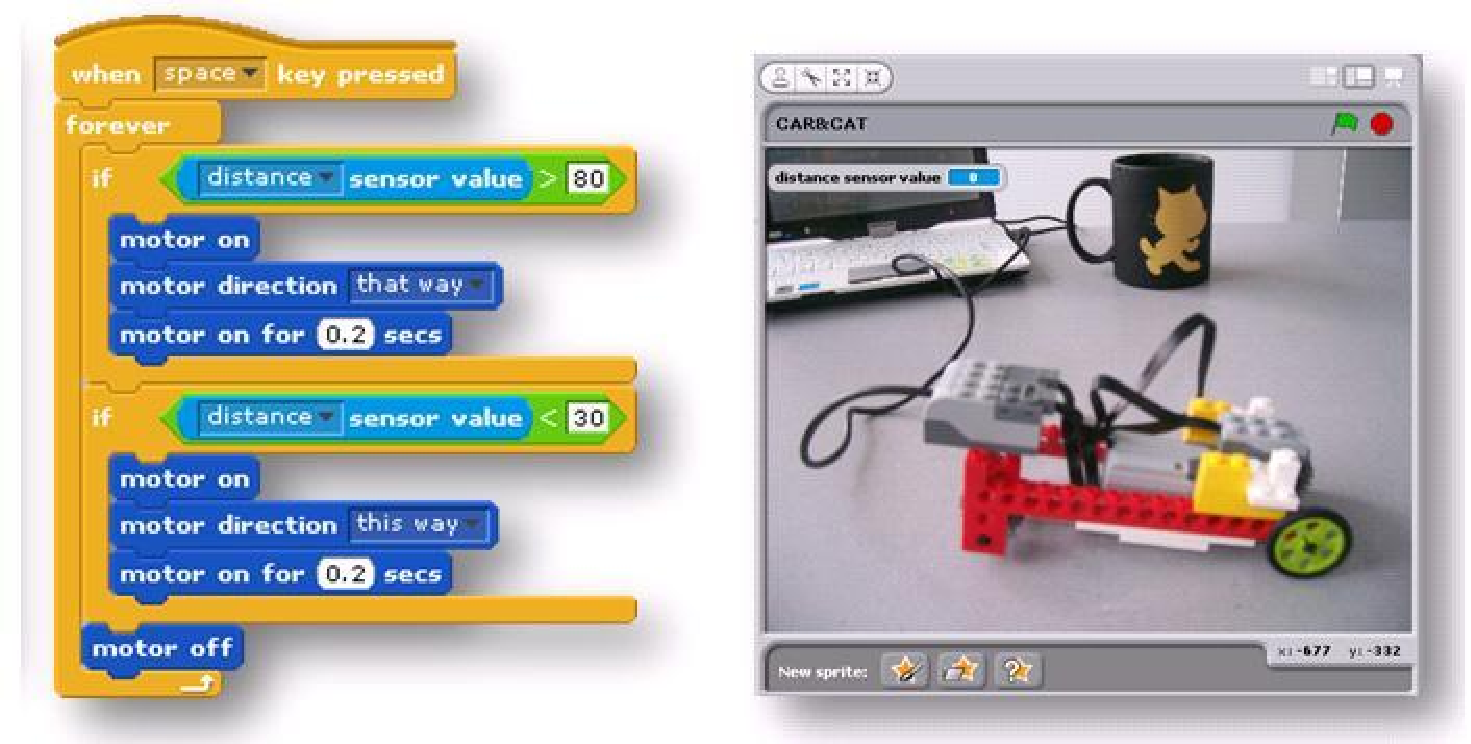
\includegraphics[width=0.5\textwidth]{ScratchWeDo.pdf}
\caption{Implementación de un automóvil autocontrolado. (Fuente: Programming and Robotics with Scratch in Primary Education \cite{ScratchWeDo})}
\label{fig:ScratchWeDo}
\end{center}
\end{figure}



Estos sistemas proporcionan al usuario un camino para avanzar en el aprendizaje hacia unos entornos de programación cada vez más complejos. Los niños pueden crear programas sencillos fácilmente, y aprender rápidamente de las interacciones físicas, preparándose para participar en el apasionante mundo de la programación de computadoras dada la interfaz correcta.



\section{Aplicaciones de sistemas multipantalla}

Este enfoque de diseño introduce una nueva experiencia multi-dispositivo, donde los distintos dispositivos se complementan entre sí, aunque hay casos en el que el usuario interactuá con los distintos elementos de manera individual, su finalidad de funcionamiento es como un grupo completo conectado, para ofrecer una experiencia mas interactiva.

La consecución de un enfoque complementario implica dos tipos de relaciones entre dispositivos:
\begin{itemize}
\item Colaboración: Cada uno de los dispositivos tienen un papel distintos entre ellos, trabajando juntos en colaboración (y normalmente simultáneamente) para construir la experiencia. Por ejemplo, jugar al domino, el tablero donde son situadas cada una de las piezas, es visualizado en un dispositivo (televisor, tablet, ordenador,…) y las fichas de cada jugador son mostradas en sus propios smartphones.

\item Control: La experiencia principal del usuario tiene lugar con un dispositivo en particular, mientras que los otros dispositivos controlan los aspectos del juego, generalmente remoto. Por ejemplo el uso de un teléfono inteligente que sirve como control remoto de una televisión.
\end{itemize}
Además, los dispositivos pueden tener un peso diferente en el conjunto del juego y son parte integral de la experiencia. 


\textbf{MPad-Controller} es una aplicación multipantalla para móviles y tablets, desarrollado por la empresa PlayMore para la compañía Apple. Se trata de un conjunto de juegos donde están implicadas varios dispositivos comunicados entre sí mediante una aplicación software, para ofrecer un entorno de juego compartido entre distintas pantallas (Figura~\ref{fig:Mpad}). Uno de los dispositivos actúa como pantalla principal para la visualización central del juego, mientras que los otros dispositivos realizan la función de joystick virtual.

\begin{figure}[!h]
\begin{center}
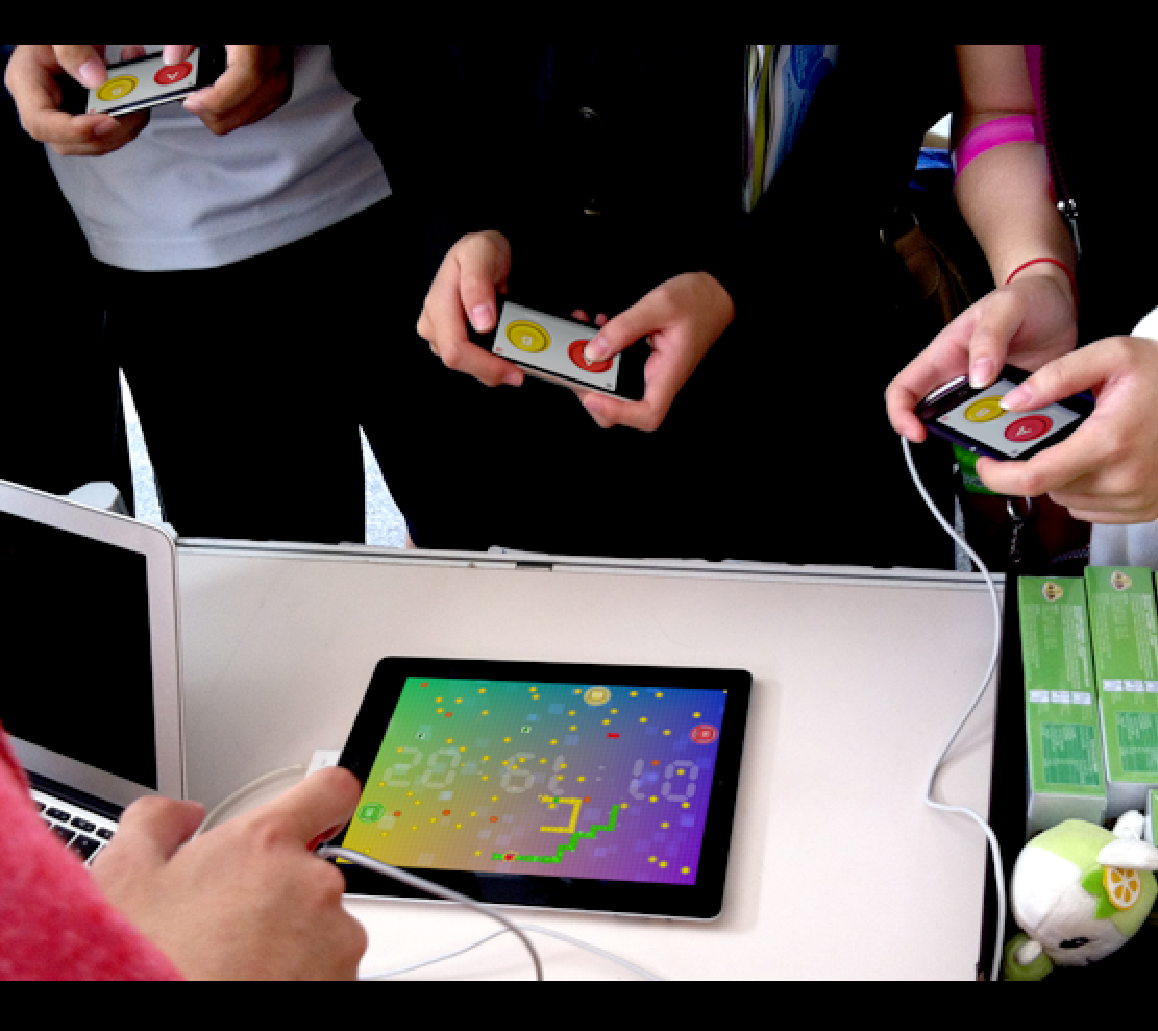
\includegraphics[width=0.5\textwidth]{Mpad.pdf}
\caption{Mpad Controller. (Fuente: PlayMore \cite{Mpad})}
\label{fig:Mpad}
\end{center}
\end{figure}


\textbf{Sifteo Cubes} \cite{Merrill}. Plataforma interactiva de juego formada por varios bloques. Cada uno posee una pantalla donde el usuario los hace interactuar entre sí cuando se agitan, inclinan, giran o se colocan unos junto a otros. Los cubos tienen un tamaño de 1,5 pulgadas y se comunican entre si a través de un protocolo de radio de 2,4 GHz. El prototipo actual soporta hasta seis cubos, y tanto la animación como la programación es efectuada mediante lenguaje C.
Este tipo de juego esta diseñados para edades a partir de 6 años.

\begin{figure}[!h]
\begin{center}
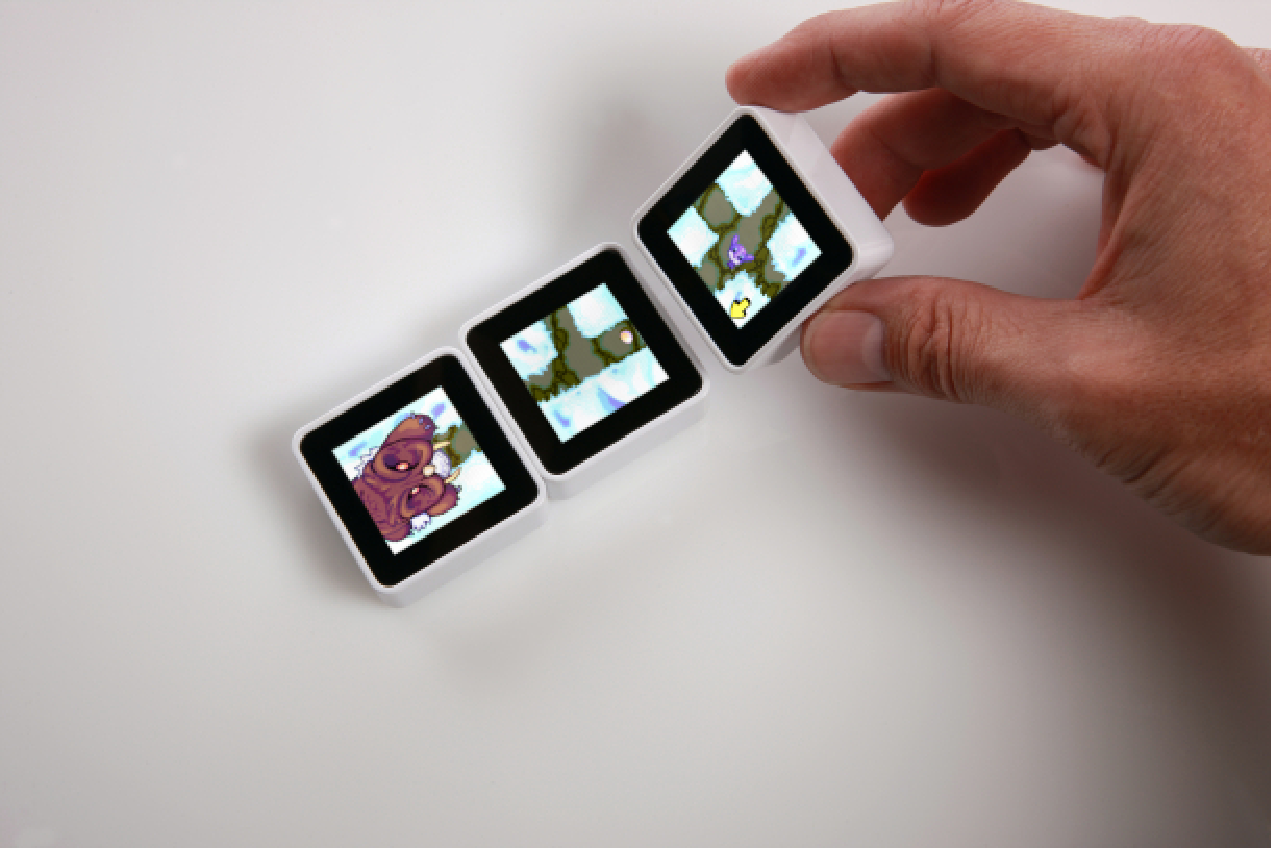
\includegraphics[width=0.5\textwidth]{Sifteo.pdf}
\caption{Sifteo Cubes. (Fuente: Sifteo Cubes \cite{Merrill})}
\label{fig:Sifteo}
\end{center}
\end{figure}

\textbf{Tangicons 3.0} \cite{Tangicons}. Este sistema pretende presentar a los niños de entre 6 y 9 años, las herramientas necesarias para fomentar el razonamiento, el trabajo colaborativo, en los primeros pasos de la programación con objetos tangibles dentro de un juego educativo. Dependiendo de los jugadores, el juego se puede actualizar con complejidad adicional para iteraciones adicionales. Promueve el razonamiento abstracto, la colaboración y la discusión entre los niños, resultando en un mejor trabajo en equipo

La primera versión de este juego estaba formada por cubos de madera no eléctricos, donde los niños debían colocarlos de forma correcta para elaborar una secuencia que finalmente accionaba un motor. Esta secuencia era reconocida mediante procesamiento de imágenes que captaba una cámara. El manejo de esta cámara fue un reto para los niños pequeños, y la transmisión entre la computadora y la estación de ejecución tampoco era muy confiable

La segunda versión integró la tecnología dentro de los cubos de programación utilizando microcontroladores ATmega8, acelerómetros y módulos de radiofrecuencia, leds, y sonido. La estación de ejecución era la encargada de alimentar a los cubos mediante una batería interna. También se le proporciono a la estación un modulo de comunicación inalámbrico para la conexión con la computadora. Uno de los juegos consistía en que los niños hicieran parejas de cubos con el mismo color. Desafortunadamente surgió el problema de que la electrónica de su interior ademas de tener un alto coste, era bastante frágil y no soportaba la rutina diaria a la que era expuesto el juego. Para solucionar estos problemas, se introdujo el uso de los cubos Sifteo.

Tangicons 3.0 busca una mezcla entre juego interactivo con el movimiento físico, es decir, los niños tienes que moverse, incluso correr entre sus tareas. Numerosos estudios muestran la relación positiva entre el movimiento y la intensidad de las habilidades intelectuales en los estudiantes. Zimmer \cite{Zimmer} demuestra  que las experiencias motrices, sirven de base para la posible creación de un “instrumento cognitivo”. Zahner \cite{Zahner} también muestra que existe una interrelación entre la actividad motora y un mayor desarrollo intelectual.

Para ejecutar uno de los juegos, los niños deben superar un laberinto donde controlan un avatar. Para hacer el recorrido del laberinto, se han de colocar los cubos en fila, en las posiciones correctas para ejecutar una correcta secuencia (Figura~\ref{fig:Tangicons}). Después de cada ciclo de ejecución, el avatar se quedará sin energía y tiene que ser “recargado”. Para recargarlo, existe una estación de recarga situada en el otro extremo del recinto donde se desarrolla el juego, por lo tanto los niños deben correr hacia esa estación junto con el cubo que representa su avatar, para poder superar correctamente el juego, manteniendo su cubo contra el cargador para posteriormente regresar a la estación de programación.

\begin{figure}[!h]
\begin{center}
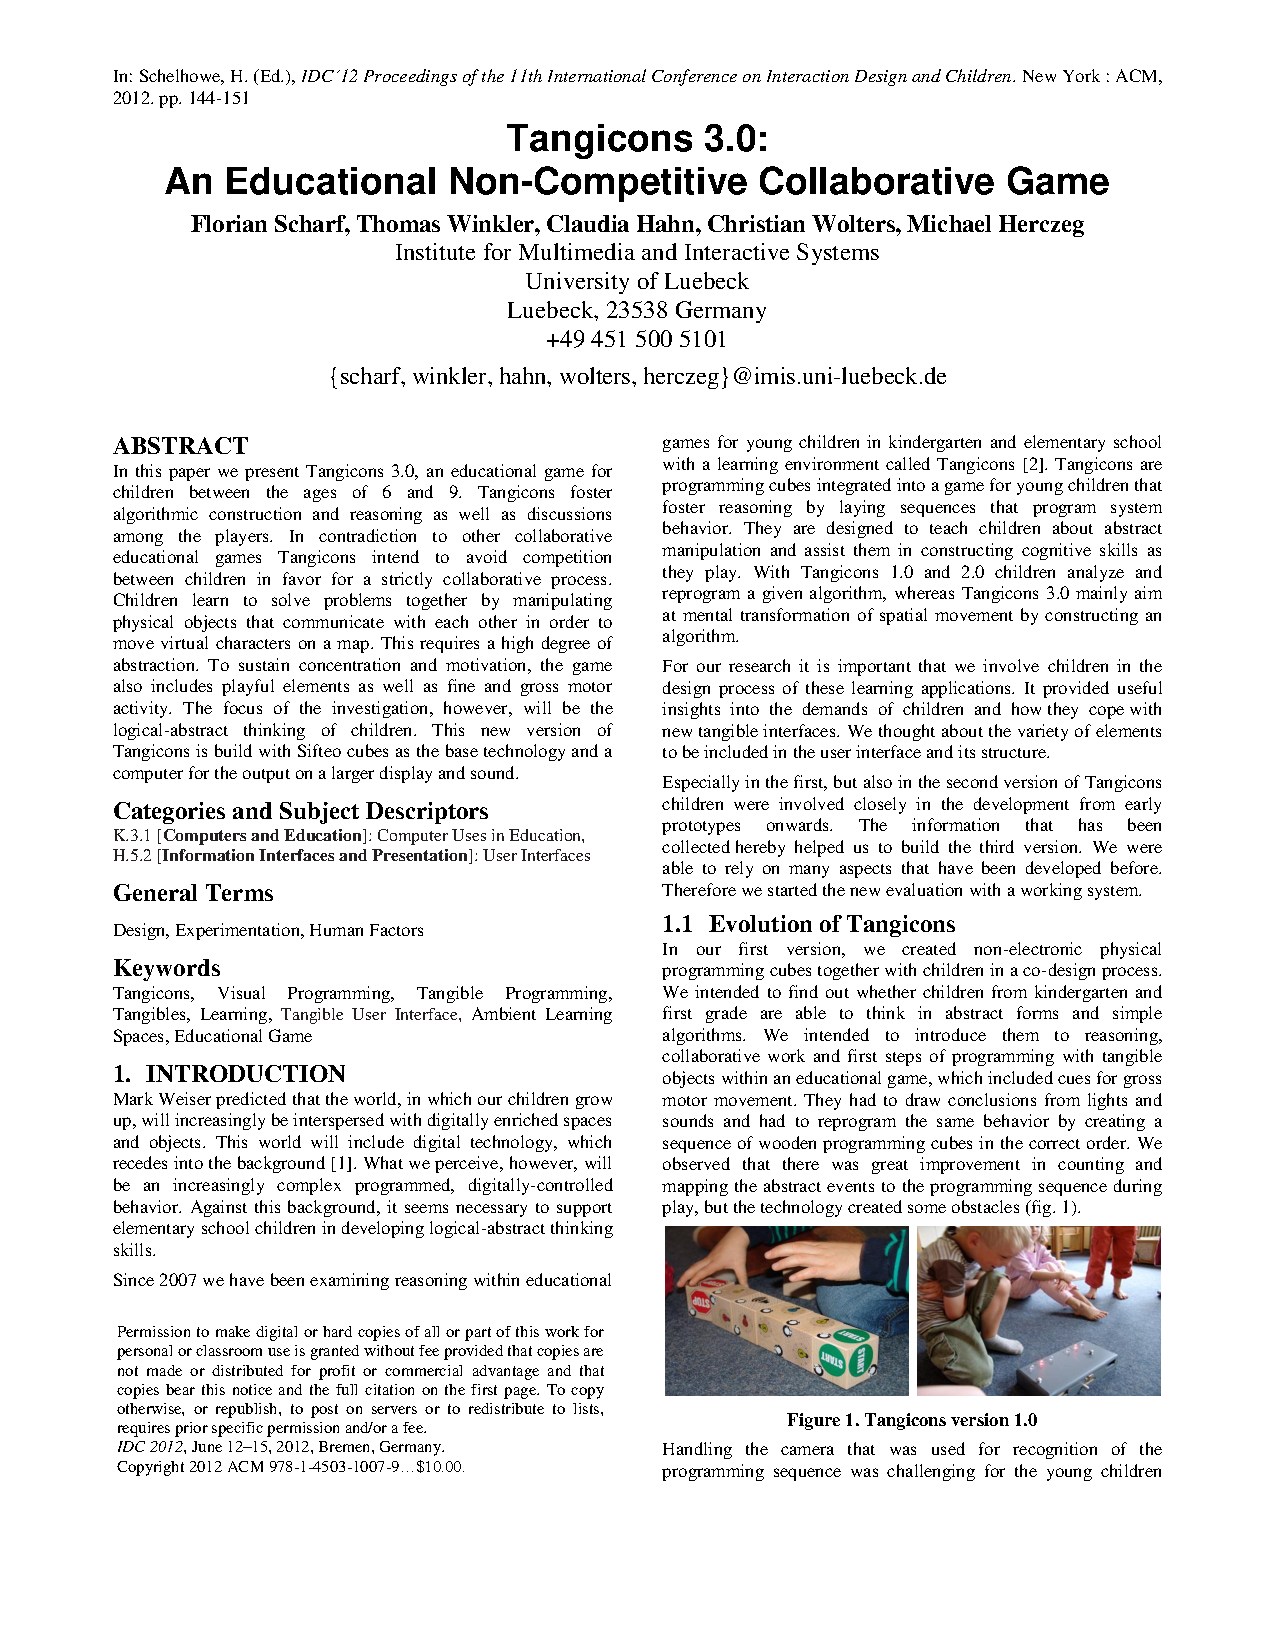
\includegraphics[width=0.5\textwidth]{Tangicons.pdf}
\caption{Tangicons versión 3,0. (Fuente: An Educational Non-Competitive Collaborative Game \cite{Tangicons})}
\label{fig:Tangicons}
\end{center}
\end{figure}



\textbf{Super Sync Sports} \cite{Awwwards} es un experimento de Google que te permite sincronizar tu teléfono móvil con tu computadora y usarlo como un controlador de juego. Consiste en varias pruebas de carácter deportivo, que los jugadores han de superar con la pantalla táctil en su dispositivo móvil. Construido con tecnologías HTML5, CSS3, Javascript y la API WebSockets, Chrome Super Sync Sports permite a hasta 4 amigos competir en juegos corriendo, nadando y en bicicleta en una pantalla de computadora compartida, usando sus smartphones o tablets como controladores de juegos (ver Figura~\ref{fig:Awwwards}) .

\begin{figure}[!h]
\begin{center}
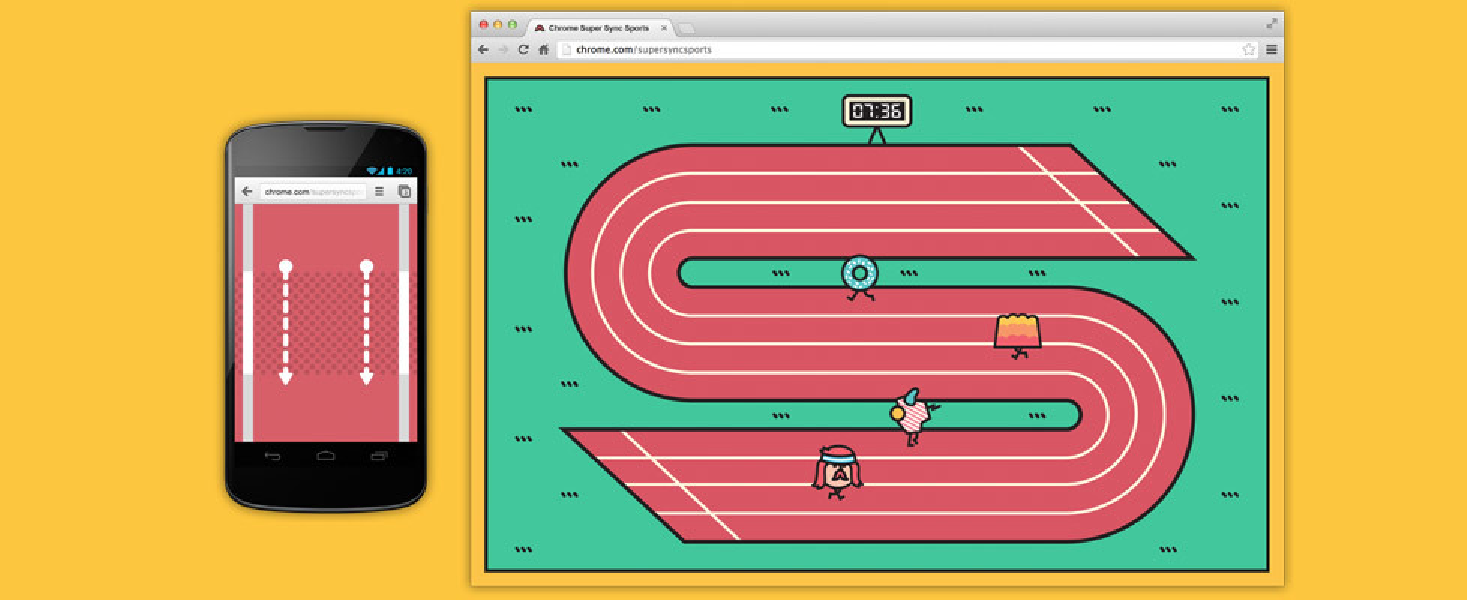
\includegraphics[width=0.5\textwidth]{Super_Sync_Sports.pdf}
\caption{Super Sync Sports. (Fuente: Awwwards \cite{Awwwards})}
\label{fig:Awwwards}
\end{center}
\end{figure}


\textbf{Pcubee} \cite{pCubee}. Diseño de una pantalla cúbica que ofrece técnicas de interacción para contenido 3D estático y dinámico. Cinco de las caras del cubo están formadas por pantallas LCD para representar imágenes en perspectiva (ver Figura~\ref{fig:pCubee}). La simulación en tiempo real simula la interacción de tener objetos reales dentro de una caja física que el usuario puede sostener y manipular. Se puede interactuar de diferentes maneras: ver una escena estática, navegar por un paisaje, jugar con objetos haciéndoles colisionar dentro del cubo y usar un lápiz para mover los objetos 3D alrededor.

\begin{figure}[!h]
\begin{center}
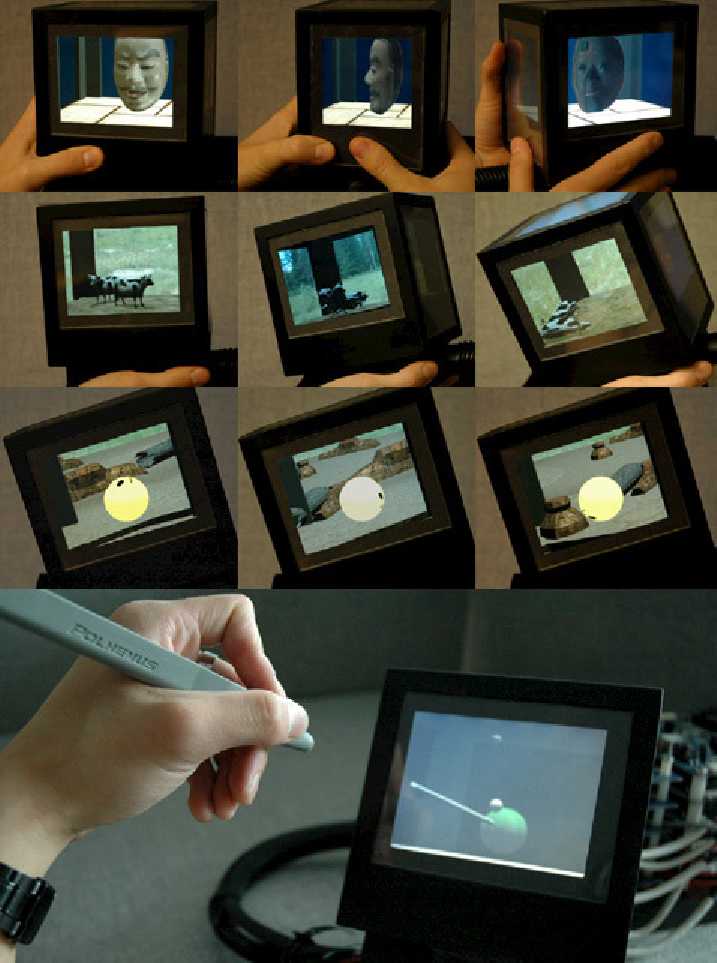
\includegraphics[width=0.3\textwidth]{pCubee.pdf}
\caption{Visualizaciones en pCubee: imagen estática, dinámica, navegación por paisaje y selección directa de objetos mediante puntero.(Fuente: pCubee: A Perspective-Corrected Handheld Cubic Display \cite{pCubee})}
\label{fig:pCubee}
\end{center}
\end{figure}





% Local Variables:
%  coding: utf-8
%  mode: latex
%  mode: flyspell
%  ispell-local-dictionary: "castellano8"
% End:
